% 翻折 引入：矩形 AB=8 BC=6, 沿对角线 AC 翻折 △ABC, B->B'
\documentclass[tikz,border=4pt]{standalone}
\usepackage{ctex}
\usepackage{amsmath}
\usetikzlibrary{calc}
\begin{document}
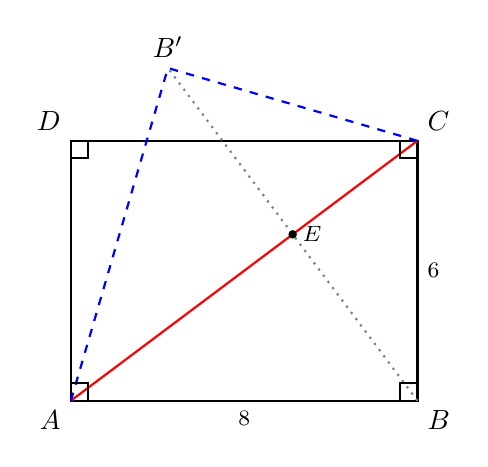
\begin{tikzpicture}[scale=0.55, thick]
  % A=(0,0), B=(8,0), C=(8,6), D=(0,6). AC 为折痕
  \coordinate (A) at (0,0);
  \coordinate (B) at (8,0);
  \coordinate (C) at (8,6);
  \coordinate (D) at (0,6);
  % B 关于 AC 的对称点 B'. AC 方向 (8,6)/10. 投影 B 到 AC:
  % t = (B-A)·(C-A)/|C-A|^2 = (8*8+0*6)/100 = 64/100 = 0.64
  % 垂足 E = A + 0.64*(C-A) = (5.12, 3.84)
  % B' = 2E - B = (2.24, 7.68)
  \coordinate (E) at (5.12, 3.84);
  \coordinate (Bp) at (2.24, 7.68);
  \draw (A)--(B)--(C)--(D)--cycle;
  \draw[red] (A)--(C);
  \draw[blue, dashed] (A)--(Bp)--(C);
  \draw[gray, dotted] (B)--(Bp);
  \filldraw (E) circle (2pt);
  % 直角符号 (B 处)
  \draw ($(B)+(-0.4,0)$)--($(B)+(-0.4,0.4)$)--($(B)+(0,0.4)$);
  \draw ($(A)+(0.4,0)$)--($(A)+(0.4,0.4)$)--($(A)+(0,0.4)$);
  \draw ($(C)+(-0.4,0)$)--($(C)+(-0.4,-0.4)$)--($(C)+(0,-0.4)$);
  \draw ($(D)+(0.4,0)$)--($(D)+(0.4,-0.4)$)--($(D)+(0,-0.4)$);
  \node[below left] at (A) {$A$};
  \node[below right] at (B) {$B$};
  \node[above right] at (C) {$C$};
  \node[above left] at (D) {$D$};
  \node[above] at (Bp) {$B'$};
  \node[right] at (E) {\footnotesize $E$};
  \node[below] at ($(A)!0.5!(B)$) {\footnotesize $8$};
  \node[right] at ($(B)!0.5!(C)$) {\footnotesize $6$};
\end{tikzpicture}
\end{document}
